\documentclass{beamer}

\usepackage{apacite}



\usepackage{pgfpages}
%\setbeameroption{show notes}
%\setbeameroption{show notes on second screen=right}
\mode<presentation> {
  \usetheme{Warsaw}
  % ou autre ...

  \setbeamercovered{transparent}
  % ou autre chose (il est également possible de supprimer cette ligne)
}


\usepackage[french]{babel}


\setbeamertemplate{footline}[frame number]

\usepackage{graphicx} % Allows including images
\usepackage{booktabs} % Allows the use of \toprule, \midrule and \bottomrule in tables




\title{REVISITING HISTOGRAM}
\author
{Demudu Naganaidu (GS49320) \\
Supervisory committee: \\
Assoc Prof. Dr. Mohd Bakri Adam \\
Assoc Prof. Dr. Jayanthi Arrasan \\
Dr. Iskandar Bin Ishak }

\institute{Institute of Mathematical Research \\
University Putra Malaysia}

\date{15th May 2018}



\begin{document}

\begin{frame}
  \titlepage
\end{frame}

\begin{frame}{Outline of Presentation}
  \tableofcontents
\end{frame}

\section{Introduction}
\subsection{Histogram}
\begin{frame}{Histogram}
\begin{itemize}
	\item Exploratory Data Analysis (EDA) is an approach of analyzing data visually without a prior assumptions on parametric model of the data, error terms, outliers, modality and relationship with other variables.
	\item EDA helps the researchers to model data based on the what is revealed through exploring with various graphical methods. \item Generally after the EDA process, one would use confirmatory analysis such as hypothesis testing, ANOVA and etc.
	\item Histogram is one of the important tools used in EDA to summaries large amount data and to visualise the distribution of data.
	\item It is constructed without prior assumptions and known as nonparametric density estimator.
	
\end{itemize}
\end{frame}

\begin{frame}{Histogram (cont..)}
\begin{itemize}
		\item Once a histogram is constructed, general attributes of the data such as symmetry, modality, central location and spread of the data can be revealed.
		\item Histogram is build with stack of rectangular columns, based on frequency table which consist of intervals called bins and corresponding count of values known as frequency. Heights of column are  proportional to these frequencies.
		\item No matter how a histogram created the bins size must be decided. Bins can be either all same size (i.e same width) or different size.
		\item The number of bins determines the shape of histogram. Too many bin makes the histogram uneven and unable to find the underlying trend. Too few bin gives little information about the data.
\end{itemize}

\end{frame}
	


\subsection{Number of  Bins}
\begin{frame}{Number of Bins}
\begin{itemize}
    \item  There is no "the best" number of bins, as different bin sizes can reveal different features of the data.
	\item One usually try different bin numbers, before choosing one that illustrate the salient features of the data. \\
 	\item The number of bins k  for hisogram with equal width can determined from a suggested bin width h  or vice versa.
	$k = \Bigg[ \frac{Max(data)  - Min(data)}{h} \Bigg]$
	\item Some researchers attempted to determine an optimal number of bins by some strong assumptions on shape of the data, eg Scott(1979).
	
\end{itemize}
\end{frame}



\section{Literature Review}

\begin{frame}[allowframebreaks]{Literature Review}

\begin{itemize}
	
\item In constructing histogram, three important parameters crucial are: (i) number of bins or intervals, (ii) bin width or interval width and (iii) lower limit of first bin or interval \cite{waterman1978estimation}
	
\item In statistical theory however only few guidelines are available for selecting the number of bins or bin width for the histogram \cite   \cite[]{He1997,Lucien2006} 

\cite{Sturges1926} is one of the most cited scholar when it comes to histogram bin selection. He claims proper distribution is distributed into classes by series of binomial coefficients. Though no formal prove in this 1926 paper  was presented the number of classes, k for a dataset with N observations was written as :

\begin{equation}
k= 1 + 3.322\; log(N)
\end{equation} 


The class interval, h can be computed as: 

\begin{equation}
\large{h= \frac{R}{k} } 
\end{equation}

where R is range of data.

Sturges' add that the class interval will be useful to calculate averages, variance, skewness and other moments of frequency distributions formed with the k number of classes.

The simplicity of Sturges' formula or famously known as Sturges' rule made it as one of the most widely used formula in deciding the number classes in constructing histogram until today. Most statistical packages such as R Programming use this rule as default rule for constructing the histogram. 

Sturges' also suggest that suitable class width should be 1,2,5,10,20 or etc so that the theoretical class width, h computed from (2) can approximated to next smaller convenient class width.

\cite{Scott2009} argue that the above Sturges' formula only suitable for strictly  normal or Gausian data. He points out that data from other type of distribution require more bins  to present the distribution.

Scott derived the Sturges rule using Binomial density $ B(m,p) $ which can be approximated as normal distribution when $mp > 5$ and near normal when $p=\dfrac{1}{2}$ .

\begin{equation}
f(y)=P(Y=y)={m \choose y} p^{y}(1-p)^{m-y},
\end{equation}

\begin{center}
	$ y= 0,1,...m $
\end{center} 

\begin{center}
	when $p=\dfrac{1}{2}$ then
\end{center} 

\begin{equation}
f(y)=P(Y=y)={m \choose y}m^{-m}
\end{equation}


The bin counts, vi, given by the binomial coefficients ${m \choose i}$, for $i = 0,1, ... ,m$ giving m+1 bins. 

Number of observations n computed as 

\begin{equation}
n = \sum_{i=0}^{m} vi =  \sum_{i=0}^{m} {m \choose i} =  \sum_{i=0}^{m} {m \choose i} 1^{i} 1^{m-i} = (1 + 1)^{m} = 2^m  
\end{equation}

\begin{center}
	$log_2 n = m $ , number of bins $ k= m+ 1$ 
	
\end{center}


\begin{center}
	$ k = 1 + log_2 n $ or $ k = 1 + 3.322 log\;n $ 
\end{center}

\cite[p~605]{SCOTT1979} argue that the methods to construct histogram exist then was not  addressing problems of bias and variance in estimation. Much of intuition and past experience of the researcher plays important role. He propose new methods to construct histogram using mean squared error criteria that is more rationale.

Mean squared error of histogram estimate, $\hat{f}(x)$, of the true density value, $f(x)$, defined by

\begin{equation}
MSE(x)=\large E \left\{\hat{f}(x) - f(x)  \right\}^2
\end{equation}

Scott derived a general term for the width of the histogram as follows:

\begin{equation}
{h^*}_n =         \Bigg\{     \frac{6}{\int_{{-}\infty}^{\infty} {f'}(x)^{2} dx}  \Bigg\}^{\frac{1}{3}}n^{\frac{-1}{3}}
\end{equation}

and for Gaussian data, ${h^*}_n = 2 $ x $ 3^{\frac{1}{3}}\pi^{\frac{1}{6}}\sigma n^{\frac{-1}{3}}$

when $\sigma$ is unknown the estimate from sample, sample standard deviation is used giving the bin width,  $h_n =  3.49s n^{\frac{-1}{3}}$

\cite{Freedman1981} came out with a robust method using the Inter Quartile Range, IQR, where the bin width  ${h^*}_n =  2(IQR) n^{\frac{-1}{3}}$

\cite{Scott1985} has proposed the average shifted histogram as variation in density estimation. An algorithm by choosing m histograms but with different bin locations and averaging them to get average shifted histogram.

For a histogram with equal bin width h, and density of $f(x)$ that represent a random sample of $\left\{ x_1, ...,x_n  \right\}$. 


\cite{Brown1993} assumes that for many types of data the underlying population is normally distributed. They proposed a minimized integrated squared deviation between the histogram and normal curve. Normal curve which provides the least IMSE is used as estimate for the population mean, $\mu$ and standard deviation, $\sigma$  instead of the usual sample mean, $\bar{x}$ and sample standard deviation $s$

It is important that before fitting, histogram rescaled to ensure the area under the histogram is equal to one(1).  To do the following measures are taken:

$\xi_o = $ left endpoint of first histogram bar,

$\xi_M = $ right endpoint of last histogram bar,

$  b = $ bin width, $\xi_j = \xi_o + bj$,
$ M = (\xi_M - \xi_o )/b = $ number of histogram bins,
$ n = $ sample size, and 
$ n_j = $ number of observations in the jth bar interval.

A scaled histogram is given by 

$ h(t) = C.n_j $ if $ \xi_{j-1} < t \leq \xi_j , j = $ 1,..., M, 

with $ C = (bn)^{-1}$ to give area one.

Letting $g(.)$ denoting a nonnegative function on the line and be an area of one(1) histogram \cite{Brown1993} minimise the function $D(\mu, \sigma)$ to find the $\mu$ and $\sigma$.

\begin{equation}
D(\mu,\sigma) = \int (  \varphi_{(\mu,\sigma)} - g(t)         )^2 dt
\end{equation}

The estimated parameters $\hat{\mu}$ = $\mu^*$ and $\hat{\sigma}$ = $\sigma^*$ are reportedly quite robust.

\cite{Wand1997} regards that the bin width is the most important parameter when it comes to histograms construction. Whether a histogram is 'over smooth' or 'under smooth' is controlled by this parameter. He extended the Scott's rule to provide a simple and with asymptotic performance. However the method proposed is not straight  forward.

\cite{Bura2009} introduced the cross validation (CV) method and derived:

\begin{equation}
CV\left[h\right] = \frac{2}{h(n-1)} - \frac{n+1}{h(n-1)} \sum_{k=1}^{m}\frac{n_{2}^{k}}{n^2}
\end{equation}

where m is number of bins, $h=(x_{max} - x_{min})/m$, and $n_k$ is the $k$th bin count. The value of $h_i$ that corresponds to the minimum of CV$\left[h\right]$ defines the $h_{opt}$, optimum bin width.

\cite{CorreaM2010} cited that Freedman at. el (1978) presents a long chapter on histograms of unequal widths and their interpretations. They pointed out that, in the unequal case, the histogram represents numbers by area, but not height. They do not provide any recommendation on how to choose the limits of the classes that specify the histogram. If we choose the class limits in such a way that they correspond with some predefined percentiles, we also produce an unequal-class-width histogram, but each bar corresponds to a specific percentage of points in the sample.

The proposed using a modified histogram that is calculated from estimated deciles $ ( {\hat\xi_{\small0.1}}, {\hat\xi_{\small0.2}}.....{\hat\xi_{0.9}})$ , where  $ {\hat\xi_{\small \alpha}}$ is the estimator of  $ {\xi_{\small \alpha}}$ , and  $P (X \leq {\xi_{\small \alpha}} ) = \large{ \alpha} $ The advantage is that the number of classes is the same every time we draw a histogram and it is easy to be interpreted by the user.

One property of sample quantiles is that they are strongly consistent for the estimation of the population quantiles. This means that as the sample size increases, we are obtaining a histogram that will be closer to the histogram drawn using the true deciles. We could call this the decile histogram or decilgram. It has also been proved that,	under	mild	conditions,  $ ( {\hat\xi_{\small0.1}}$,  ${\hat\xi_{\small0.2}}.....{\hat\xi_{0.9}})$, converges	asymptotically	to	a	multi normal distribution, where $f$ is the probability density function of the data, $p=0.1, 0.2,...,0.9,$ and $n$ is the sample size.


Now, for $0<p_{1} < p_{2} <...p_{k} < 1$, assessing that $f$ is positive and continuous in a boundary of $\xi_{p_{1}}, \xi_{p_{2}},...,\xi_{p_{k}} $, then $\bigg(\hat{\xi_{p_{1}}}, \hat{\xi_{p_{2}}},...,\hat{\xi_{p_{k}}} \bigg)$ is asymptotically	normal	with		mean	vector  $(\xi_{p_{1}}, \xi_{p_{2}},...,\xi_{p_{k}}) $ and covariance $\sigma_{ij}/n$, where 

\begin{equation}
\sigma_{ij}=\frac{p_{i}(1-p_{j})}{f(\xi_{p_{i}})f(\xi_{p_{j}})}
\end{equation}

for $i \leq j$ , and $\sigma_{ij} = \sigma_{ji}$ for $i>j$ 

\cite{NurhanDoganAfyon2016} listed bibliography of 23 methods that can be used for determination of bins used in histogram and frequency tables. They cited there are too many recommendations. 14 methods were used to determine number of bins based on simulated data. It is concluded that number of bins not only  depends number of observations $n$ but also depends on the range of the data. In general \cite{NurhanDoganAfyon2016} recommended minimum but not more than 15 bins are used. 

\cite{Gunver2017} argue that current method namely Scott (1979) or Freedman -Diaconis (1981) rules that contain $ \hat{s}$ and/or n, can cause variant histogram peaks due to skewness and/or sample size data stacks. They proposed percentile based bin width histogram which is more robust irrespective of sample size and skewness and standard deviation. \cite{Gunver2017} claims histogram generated by their method able to make anomalies in stack data.

\end{itemize}

\end{frame}

\section{Problem Statement}

\subsection{Unequal Bin Width Histogram}
\begin{frame}{Problem Statement}
	\begin{itemize}
		\item Freedman at el (1978), presented in detail on unequal histogram and their interpretations. 
                     \item In unequal bin width the  histogram represents numbers by area, but not by height.
		\item However they did not provide any recommendation on how to choose the different limits for each unequal bin width.
	\end{itemize}
\end{frame}

\begin{frame}{Example of Unequal Width Histogram}

\begin{figure}[t]
       	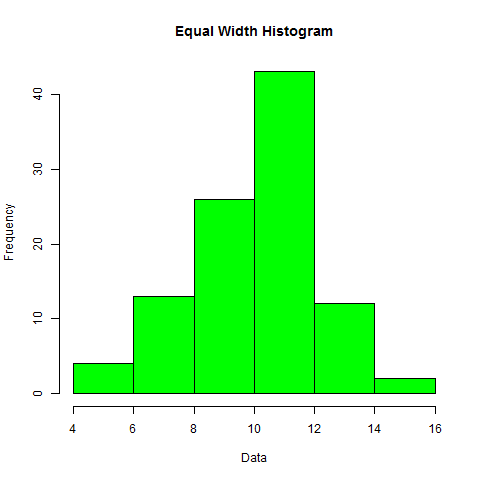
\includegraphics[width=2in]{equal}
  \centering
\end{figure}
All interval are with unequal width. The vertical axis provide density for each interval. Here the area for each bar is important.
\end{frame}

\section{Method}

\subsection{The Modified Histogram}

\begin{frame}{The Modified Histogram}
	\begin{itemize}
		\item We propose the class limits in such a way that they correspond with some predefined percentiles.
		\item Such class limits also produce an unequal class width histogram.
 		\item We could use a modified histogram that is calculated from estimated deciles $ ( {\hat\xi_{\small0.1}}, {\hat\xi_{\small0.2}}.....{\hat\xi_{0.9}})$ , where  $ {\hat\xi_{\small \alpha}}$ is the estimator of  $ {\xi_{\small \alpha}}$ , and  $P (X \leq {\xi_{\small \alpha}} ) = \large{ \alpha} $ 

		\item Sample quantiles are consistant estimator of population quantiles (Serfling,1980). The similar way as sample size increases we are obtaining histogram that will be closer to the histogram drawn using the true deciles.

	\end{itemize}
\end{frame}

\section{Results}
\begin{frame}{Results}
	\begin{itemize}
		\item For illustrations of above idea, several histograms drawn using the dataset for times that long distance runners spent in the Medellin 2009 Half Marathon Race. 
		\item It is known that runners conform to well defined groups.
	\end{itemize}
\end{frame}

\subsection{Commmon Histograms}
\begin{frame}{Common Histograms}

	\begin{figure}[t]
		\centering
       		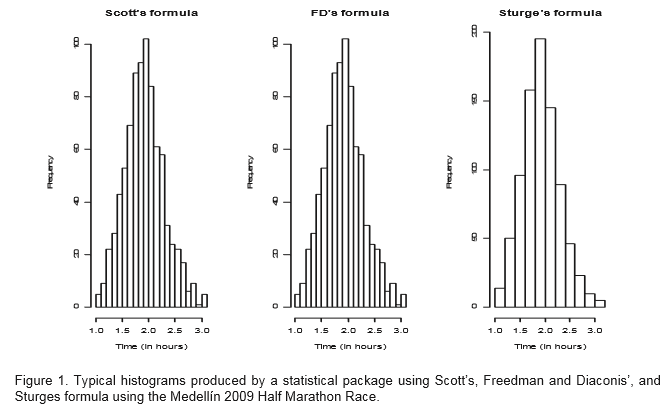
\includegraphics[scale=0.6]{figure1}
 
	\end{figure}

\end{frame}


\subsection{Decile Histogram}
\begin{frame}{Decile Histogram}

	\begin{figure}[t]
		\centering
       		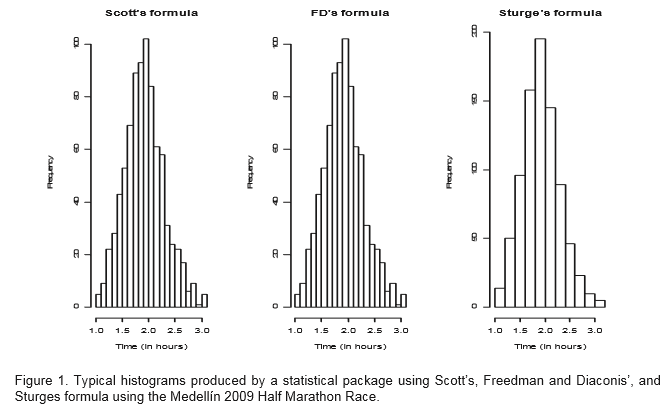
\includegraphics[scale=0.65]{figure1}
 
	\end{figure}

\end{frame}


\subsection{Quartile Histogram}
\begin{frame}{Comparing Quartile Histogram with Boxplot}

	\begin{itemize}
		\item We choose limits of classes of a histogram based on 5 number summary used to construct boxplot.
		\item Histogram drawn has the same meaning of boxplot corresponds to quartile histogram.
		
	\end{itemize}

\end{frame}

\begin{frame}{Quarile Histogram- Using 5 number Summary}

	\begin{figure}[t]
		\centering
       		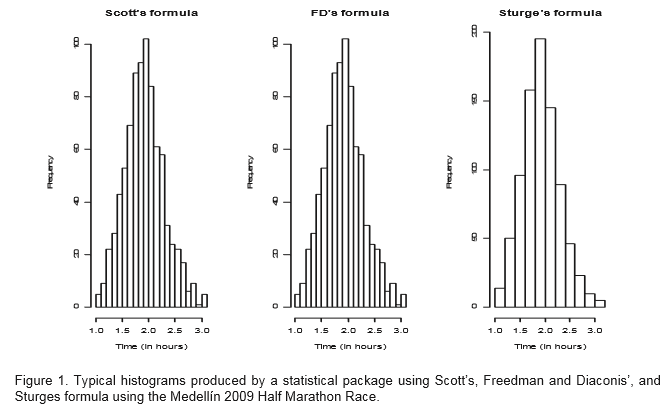
\includegraphics[scale=0.65]{figure1}
 	\end{figure}
However the plot hides the modality of the data when exist (Fridge at el, 1989).
\end{frame}

\section{Conclussion}
\begin{frame}{Conclussion}
	\begin{itemize}
			\item We can modify the current histogram to Decile histogram to provide more information.
			\item The limits of the classes are point estimators of the real limits. 
			\item For future research we can consider new class of histogram in which limits of bars are confidence intervals containing the actual ones.
			\item The current histogram lose some characteristics of the distribution, such as number of the data per class and we need boxplot to analyse the whole data.
			\item Quartile histograms hides the multimodality, thus researcher must look for other kind of boxplot.

	\end{itemize}

\end{frame}


\begin{frame}[allowframebreaks]
\frametitle{References}
\begin{enumerate}
	\setcounter{enumi}{0}
	\item Beniger, J. R. and Robyn, D. L. (1976). The history and future of graphics in statistics. Social Statistics Proceedings, pages 192 - 197. 
	\item Berger, M. A., Mathew, P. A., andWalter, T. (2016). Big data analytics in the building industry.ASHRAE Journal, 58(LBNL–1005983).
	
\end{enumerate}
\end{frame}

\subsection{Bibliography}
\begin{frame}[allowframebreaks]{References}
\tiny
\bibliographystyle{apacite}
\bibliography{bibbliografi}
\end{frame}
\end{document}